
\section{Preliminaries}\label{sec:vanilla}
%---------------------------------------------------------------------------------------------------%
% Things to put here:
% - A bit of computational and complexity introduction
% - Finite fields and arithmetic circuits
% - R1CS
% - QAP
% - Hash functions
% - Tree modes
%---------------------------------------------------------------------------------------------------%
In this section we are going to introduce some fundamental concepts;
while some are relatively basic and wide-known, it can still be useful to skim over them to be sure
of having a firm grasp on the main ideas behind ZK-SNARK systems.

\subsection{Computational models and complexity}
A \emph{computational model} (or model of computation) is any kind of `device', either physical or
mathematical, which is able to compute algorithms to solve problems.
A particularly interesting class of problems are \emph{decision problems}, the ones that can be
answered with `yes' (or `accept', or \(\top \)) or `no' (or `reject', or \(\bot \)).
Every computational model is able to \emph{decide} only a subclass of all decision problems, and
even then, not all can be solved \emph{efficiently}, that is, by using an amount of resources
(tipically, time and space) which is upper-bounded by some polynomial function of the input length.
Problems for which a polynomial bound doesen't exist or isn't known are said to be \emph{hard} for
the computational model.
For example, finding solutions to boolean equations (the \textsc{sat} problem) is believed to be
hard for deterministic Turing machines, but it is easy for non-deterministic ones.
Unfortunately, non-deterministic Turing machines (along with any other non-deterministic model of
computation) are more of a mathematical tool than anything, and there seems to be no practical way
to efficiently solve the problems which would take Non-deterministic Polynomial time (NP-complete 
problems) as stated by the strong Church-Turing thesis.
While it is widely belived that efficiently solving NP-complete problems is impossible, there are 
some problems which lie in a `gray zone' between \textsc{NP-complete} and \textsc{P} (i.e.\ 
problems which can be solved in deterministic polynomial time): they are believed to be hard for 
deterministic models (hence, they are not in \textsc{P}), but there is no proof that they are 
\textsc{NP-complete}.
The most famous of such problems is factorization: with the advent of quantum-computing, 
which challenges the strong Church-Turing thesis, Shor devised an efficient quantum algorithm 
for factorizing numbers.
While still far from usable in practical cases, its existence proves that one must be extremely
careful when talking about the hardness of problems, especially when applied to cryptography, 
and must always make clear assumptions on the underlying model of computation.

\subsection{Fields and groups}
While computational models tipically operate over binary strings, that is, elements of
\({\{0, 1\}}^*\), where \(*\) indicates Kleene's closure, we often want to interpret such strings
as elements of some algebraic structure.
\begin{definition}
	A \emph{field} is any triple \(\mathbb{F} = (F, \oplus, \otimes)\), where \(F\) is called
	\emph{underlying set}, \(\oplus\colon F \times F \mapsto F\) is called \emph{field addition} and
	\(\otimes\colon F \times F \mapsto F\) is called \emph{field multiplication}, such that both
	addition and multiplication are commutative and associative, multiplication
	distributes over addition, \(F\) contains an additive identity element \(0_{\mathbb{F}}\) and a
	multiplicative identity element \(1_{\mathbb{F}}\), \(\forall x \in F\) there is an additive inverse
	element \(-x\), and \(\forall x \in F\setminus \{0_{\mathbb{F}}\} \) there is a multiplicative
	inverse
	element \(x^{-1}\).
\end{definition}

\noindent For example, \(\mathbb{R}\) and \(\mathbb{C}\) are fields, as is Boole's algebra
\(\mathbb{B} = (\{0, 1\}, \textsc{xor}, \textsc{and})\).
We denote elements of a field \(\mathbb{F}\) (abusing notation, as they are actually
elements of the underlying set \(F\)) with lowercase letters \(a, b, c\dots \) and variables over
\(\mathbb{F}\) with lowercase letters \(x, y, z\dots \).

If \(|\mathbb{F}| \in \mathbb{N}\), then \(\mathbb{F}\) is a \emph{finite field}.
We are particularly interested in finite fields of the kind:
\[\mathbb{F}_{p^k} = (\{0, \dots, p^k-1\}, \oplus_p, \otimes_p)\]
where \(p\) is a prime and \(\oplus_p, \otimes_p\) denote addition and
multiplication modulo \(p\) (for example, \(\mathbb{B} = \mathbb{F}_2\)).
Tipically, we consider \(n\)-bit strings either as elements of \(\mathbb{F}_{2^n}\) or of
\(\mathbb{F}_{p^1}\), where \(\log_2(p) \approx n\).
We will often use \(+\) in place of \(\oplus_p \) when denoting addition and omit \(\otimes_p \)
when denoting multiplication, if \(\mathbb{F}\) is clear from the context.

Any field \(\mathbb{F}\) can be extended to an \(n\)-dimensional vector space
\(\mathbb{F}^n\), for some \(n \in \mathbb{N}\).
We denote vectors in \(\mathbb{F}^n\) with lowercase bold letters (\(\bm{v}, \bm{w}, \dots \)), and
the \(i\)th element of a vector \(\bm{v}\) with \(\bm{v}_i\).
Vector operations follow their natural definitions depending on the underlying field.
We can also introduce matrices over \(\mathbb{F}^{n \times m}\) for some \(n, m \in \mathbb{N}\),
which we denote with bold capital letters (\(\bm{A}, \bm{B}, \dots \)).
The \(i\)th row of a matrix \(\bm{M}\) is denoted with \(\bm{M}_i\), and the \(j\)th element of
the \(i\)th row is denoted with \(\bm{M}_{i,j}\).
Matrix operations also follow their natural definitions over the underlying field.
Given \(\bm{A} \in \mathbb{F}^{n \times m}, \bm{B} \in \mathbb{F}^{n \times m'}\),
we denote with \(\begin{pmatrix}\bm{A} & \bm{B}\end{pmatrix}\) their concatenation along the rows,
and with \(\begin{pmatrix}\bm{A}; \bm{B}\end{pmatrix} =
{\begin{pmatrix}{\bm{A}}^{\transpose} & {\bm{B}}^{\transpose}\end{pmatrix}}^{\transpose}\)
their concatenation along the columns.

A field \(\mathbb{F}\) can also be extended to a monovariate polynomial ring \(\mathbb{F}[x]\),
we will denote polynomials with lowercase letters (\(p, q, \dots \)).
Operations over polynomials are naturally derived from the underlying field.
Vectors and matrices of polynomials are denoted with the usual notation
(\(\bm{p}, \bm{q}, \dots\) and \(\bm{P}, \bm{Q}, \dots\)).

Given some \(\bm{x}, \bm{y} \in \mathbb{F}^n\), we can build the unique polynomial:
\[p \mid {p \in \mathbb{F}[x]} \land {\deg(p) = n-1} \land {\forall i\colon p(\bm{x}_i) = \bm{y}_i}\]
by using Lagrange interpolation:
\[
	p = L(\bm{x}, \bm{y}) =
	\sum_{i}{\bm{y}_{i}\prod_{j \neq i}{\frac{x - \bm{x}_j}{\bm{x}_i - \bm{x}_j}}}
\]
We can extend Lagrange interpolation to any pair of matrices
\(\bm{X}, \bm{Y} \in \mathbb{F}^{n\times m}\) by applying \(L\) to every row:
\[L(\bm{X}, \bm{Y}) = (L(\bm{X}_1, \bm{Y}_1) \dots, L(\bm{X}_n, \bm{Y}_n)) \]

\begin{definition}
	A \emph{group} is a pair \(\mathbb{G} = (G, \odot)\), where \(G\) is called \emph{underlying set},
	and \(\odot\colon G \times G \mapsto G\) is called \emph{group composition}, such that
	composition is associative, there is a compositive identity element \(1_{\mathbb{G}}\), and
	\(\forall x \in \mathbb{G}\) there is a compositive inverse \(x^{-1}\).
\end{definition}

\noindent For example, \(\mathbb{Z}\) with only addition is a group (where \(1_{\mathbb{Z}} = 0\)),
as is \(\mathbb{Q}\) with only multiplication and without \(0\) (as it's not invertible).
We denote elements and variables over groups in the same way we do for fields.
We can define \emph{group exponentiation} following the natural definition:
\[\forall x \in \mathbb{G}, \forall n \in \mathbb{N}\colon x^n = \bigodot^{n}{x}\]

Any group \(\mathbb{G}\) for which \(|\mathbb{G}| \in \mathbb{N}\) is a \emph{finite group}.
We can build a finite group from a \emph{generator} set \(S\) and a composition operation
\(\odot \) by closing \(S\) under \(\odot \):
\begin{align*}
	 & {\langle{S}\rangle}^i =
	\begin{cases}
		S                                                                                   & i = 0
		\\
		{\langle{S}\rangle}^{i-1} \cup \{x \odot y \mid x,y \in {\langle{S}\rangle}^{i-1}\} & i > 0
		\\
	\end{cases}
	\\
	 & \mathbb{G} = \langle{S}\rangle =
	(\min_{i}{{\langle{S}\rangle}^{i}} \mid {\langle{S}\rangle}^{i} = {\langle{S}\rangle}^{i-1}, \odot)
\end{align*}
We are particularly interested in \emph{cyclic groups}, i.e.\ finite groups of the type
\(\mathbb{G}_q(g) = \langle{g}\rangle = ({\{g^i \bmod q\}}_{i \in \mathbb{N}},
\otimes_q)\), where \(g \in \mathbb{F}_p\) is called \emph{generator element} and
\(\mathbb{F}_p\) is called \emph{underlying field}.
Since every element of \(\mathbb{G}_q(g)\) is obtained by exponentiating \(g\), we can define a
bijective \emph{discrete logarithm} function:
\[\log_g\colon \mathbb{G}_q(g) \mapsto \mathbb{F}_p = \{(x, y) \mid x = g^y\} \]
Cyclic groups are very interesting because, while it's easy to compute exponentiation, no
deterministic algorithm is known that can efficiently compute the discrete logarithm.
\begin{definition}
	Given cyclic groups \(\mathbb{G}_1, \mathbb{G}_2, \mathbb{G}_{\transpose}\), a
	\emph{bilinear map} is any function:
	\[B\colon \mathbb{G}_1 \times \mathbb{G}_2 \mapsto \mathbb{G}_{\transpose} \mid
		\forall x \in \mathbb{G}_1, \forall y \in \mathbb{G}_2, \forall a,b \in \mathbb{Z}\colon
		B(x^a, y^b) = {B(x, y)}^{ab}\]
	If \(|\mathbb{G}| = |\mathbb{G}'|\), then \(B\) is \emph{order-preserving}, and if
	\(\mathbb{G}_1 = \langle{g_1}\rangle \land \mathbb{G}_2 = \langle{g_2}\rangle \land
	\mathbb{G}_{\transpose} = \langle{B(g_1, g_2)}\rangle \), then \(B\) is \emph{admissible}.
\end{definition}

\noindent We are interested in (order-preserving, admissible) bilinear maps where
\(\mathbb{G}_1 = \mathbb{G}_2 = \mathbb{G}\).
Bilinar maps have many application in cryptography, as they are an essential tool to exploit the 
hardness of the discrete logarithm problem.


\subsection{Arithmetic Circuits}
A sequence of operations over field elements and variables can be neatly represented by
\emph{arithmetic circuits}.
\begin{definition}[Arithmetic circuit]
	Given a field \(\mathbb{F}\), some \(n, m \in \mathbb{N}\), some constants
	\(a_{1, 1}, \dots, a_{m, n} \in \mathbb{F}\), and some variables \(x_1, \dots, x_n \) over
	\(\mathbb{F}\), an \emph{implicit arithmetic circuit} over \(\mathbb{F}\) is any formula:
	\begin{align*}
		 & \phi \equiv c                     &  & \textnormal{with \(c \in \mathbb{F}\)}
		\\
		 & \phi \equiv x                     &  & \textnormal{with \(x\) variable over
			\(\mathbb{F}\)}
		\\
		 & \phi \equiv \phi_1^c              &  & \textnormal{with \(c \in \mathbb{F}\) and
			\(\phi_1 \neq \phi \) arithmetic circuit}
		\\
		 & \phi \equiv \phi_1 \oplus \phi_2  &  & \textnormal{with \(\phi_1 \neq \phi, \phi_2 \neq
			\phi \)
			arithmetic circuits}
		\\
		 & \phi \equiv \phi_1 \otimes \phi_2 &  & \textnormal{with \(\phi_1 \neq \phi, \phi_2 \neq
			\phi \)
			arithmetic circuits}
		\\
		 & \phi \equiv \phi_1, \phi_2        &  & \textnormal{with \(\phi_1 \neq \phi, \phi_2 \neq
			\phi \)
			arithmetic circuits}
	\end{align*}
	An arithmetic circuit which does not contain multiplications and exponentiations by constants
	is called \emph{explicit arithmetic circuit}.
\end{definition}

\noindent Every arithmetic circuit can be represented by a Directed Acyclic Graph (DAG),
where the vertices are labeled either with a variable name (\emph{variable vertices}), a constant
from the field (\emph{constant vertices}) or one of the operations \(\oplus \)
(\emph{addition vertices}, denoted \(\phi_\oplus \)) and \(\otimes \) 
(\emph{multiplication vertices}, denoted \(\phi_\otimes \)).
With an analogy to digital circuits, vertices are also called \emph{gates}.
Only addition and multiplication vertices have incoming edges (exactly two), which represent the
inputs of the operation, while the outgoing edge will represent the result.
Vertices without incoming edges are called \emph{input vertices}, while vertices without outgoing
edges are called \emph{output vertices}, together they are denoted \(\phi_{IO}\).

It is possible, without affecting the expressive power, to transform an implicit arithmetic circuit
into an explicit one by replacing exponentiations (multiplications) by some constant \(c\) with a
a sequence of \(c\) multiplications (additions)\footnote{However, this transformation can affect
	the succinctness of a circuit and its DAG (unrolling \(x^c\) or \(cx\) requires \(\Theta(2^c)\)
	space), but this won't be a problem for us.}.
\begin{figure}
	\centering
	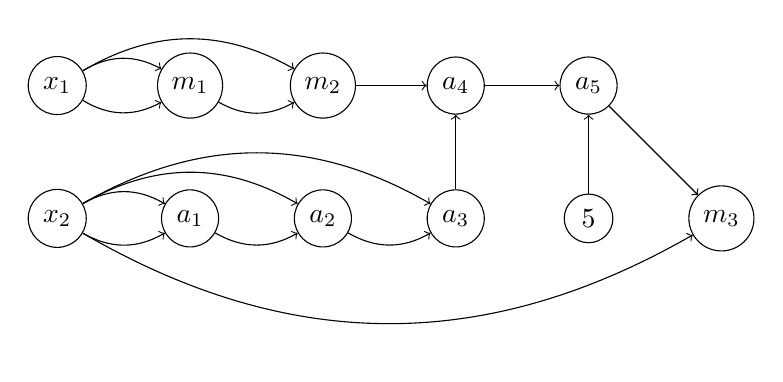
\begin{tikzpicture}[node distance={48pt}, node/.style = {draw, circle}]
		\node[node] (x1) {\(x_1\)};
		\node[node] (x2) [below of=x1] {\(x_2\)};
		\node[node] (m1) [right of=x1] {\(m_1\)};
		\node[node] (m2) [right of=m1] {\(m_2\)};
		\node[node] (a1) [right of=x2] {\(a_1\)};
		\node[node] (a2) [right of=a1] {\(a_2\)};
		\node[node] (a3) [right of=a2] {\(a_3\)};
		\node[node] (a4) [right of=m2] {\(a_4\)};
		\node[node] (a5) [right of=a4] {\(a_5\)};
		\node[node] (5) [below of=a5] {\(5\)};
		\node[node] (m3) [right of=5] {\(m_3\)};
		\draw[->] (x1) to [bend left] (m1);
		\draw[->] (x1) to [bend right] (m1);
		\draw[->] (x1) to [bend left] (m2);
		\draw[->] (m1) to [bend right] (m2);
		\draw[->] (x2) to [bend left] (a1);
		\draw[->] (x2) to [bend left] (a2);
		\draw[->] (x2) to [bend left] (a3);
		\draw[->] (x2) to [bend right] (a1);
		\draw[->] (a1) to [bend right] (a2);
		\draw[->] (a2) to [bend right] (a3);
		\draw[->] (m2) to (a4);
		\draw[->] (a3) to (a4);
		\draw[->] (a4) to (a5);
		\draw[->] (5) to (a5);
		\draw[->] (a5) to (m3);
		\draw[->] (x2) to [bend right] (m3);

	\end{tikzpicture}
	\caption{DAG of the circuit in Example~\ref{ex:circuit}.
		We have the two variable/input vertices \(x_1\) and \(x_2\), the constant vertex \(5\), the
		addition vertices \(a_1, \dots, a_5\) and the multiplication vertices \(m_1, m_2\) and
		\(m_3\),
		which is also an output vertex.}\label{fig:example_dag}
\end{figure}
\begin{example}\label{ex:circuit}
	Let's consider the following implicit arithmetic circuit over \(\mathbb{F}_{13}\):
	\[\phi = x_{2}\left(x_{1}^{3} + 4x_{2} + 5\right)\]
	We can unroll it into an equivalent (explicit) arithmetic circuit:
	\[\widehat{\phi} = x_{2}\left(x_{1}x_{1}x_{1} + x_{2} + x_{2} + x_{2} + x_{2} + 5\right)\]
	And draw the associated DAG, which is shown in Figure~\ref{fig:example_dag}.
\end{example}

\subsection{Rank-1 Constraint systems}
Like it happens for boolean formulae and the famous \textsc{sat} problem, arithmetic circuits can
also be seen as a form of constraint whose solution is a set of valid assignments for all the
intermediate values in the computation.
\begin{definition}[Rank-1 Contraint System]
	Given a field \(\mathbb{F}\) and some \(m, n \in \mathbb{N}\), a
	\emph{\(n/m\) Rank-1 Constraint System (R1CS)} over \(\mathbb{F}\) is any triple:
	\[\mathcal{C} = \left(\bm{A}, \bm{B}, \bm{C}\right) \mid \bm{A}, \bm{B}, \bm{C} \in \mathbb{F}^{n
			\times m} \]
	A \emph{solution} to some R1CS \(\mathcal{C}\) is any (column) vector:
	\[\bm{s} \mid \bm{s} \in \mathbb{F}^m \land
		\left(\bm{A}\bm{s}\right)\left(\bm{B}\bm{s}\right) = \bm{C}\bm{s} \]
\end{definition}

\noindent Any explicit arithmetic circuit with \(n\) multiplicative gates and \(m\) variables
\(x_1, \dots, x_n\) can be associated with an \(n/\left(n+m+1\right)\) R1CS \(\mathcal{C}\) which
represents the constraints in the circuit, roughly in the following way:
\begin{enumerate}
	\item Add a new `constant variable' which always assumes value \(1\).
	\item For every multiplicative gate \(\otimes_i \) in the circuit, add a new \emph{intermediate}
	      variable \(t_i\) (\(t_n\) can be denoted \(y\) as it represents the circuit output).
	\item Define the column vector
	      \(\bm{x} = {\begin{pmatrix}1 & x_1 & \cdots & x_m & t_1 & \cdots & t_n
	      \end{pmatrix}}^\transpose \).
	\item Express every multiplication gate \(\otimes_i \) as an equation in the canonical form:
	      \[\left(\bm{a_i}\bm{x}\right)\left(\bm{b_i}\bm{x}\right) = \bm{c_i}\bm{x}\]
	      where \(\bm{a_i}\) \(\bm{b_i}\) \(\bm{c_i}\) will be the \(i\)th rows of
	      \(\mathcal{C}_{\bm{A}}\), \(\mathcal{C}_{\bm{B}}\) and \(\mathcal{C}_{\bm{C}}\) respectively.
\end{enumerate}

\noindent Let's make an example to better understand the process.
\begin{example}\label{ex:r1cs}
	Consider the explicit arithmetic circuit over \(\mathbb{F}_{13}\) of Example~\ref{ex:circuit}:
	\[\widehat{\phi} = x_2\left(x_1x_1x_1 + x_2 + x_2 + x_2 + x_2 + 5\right)\]
	We can see that there are a total of 3 multiplications in the circuit, and since we have two input
	variables, our associated R1CS will be a \(3/6\) R1CS (\(2+1+3 = 6\)).
	Let's explicit all of the intermediate variables:
	\begin{align*}
		 & t_1 = x_1x_1 &  & t_2 = t_1x_1 + 4x_2 + 5 &  & y = t_2x_2
	\end{align*}
	So, our variable vector will be:
	\[\bm{x} = \begin{pmatrix}1 & x_1 & x_2 & t_1 & t_2 & y\end{pmatrix}\]
	Now, let's transform all the equations in canonical form:
	\begin{align*}
		 & \left(x_1\right)\left(x_1\right) = t_1                   \\
		 & {\left(t_1\right)\left(x_1\right) + 4x_2 + 5 = t_2} \iff
		{\left(t_1\right)\left(x_1\right) = 8 + 9x_2 + t_2}         \\
		 & \left(x_2\right)\left(t_2\right) = y
	\end{align*}
	Remember that we are working over \(\mathbb{F}_{13}\), so in the second equation, when we bring
	\(4\) and \(8\) to the right side, we have \(-4 \equiv 9 \pmod{13}\) and \(-5 \equiv 8 \pmod{13}\).
	We can now extract our R1CS \(\mathcal{C} = \left(\bm{A}, \bm{B}, \bm{C}\right)\):
	\[
		\mathcal{C} =
		\left(
		\begin{pmatrix}
				0 & 1 & 0 & 0 & 0 & 0 \\
				0 & 0 & 0 & 1 & 0 & 0 \\
				0 & 0 & 0 & 0 & 1 & 0
			\end{pmatrix},
		\begin{pmatrix}
				0 & 1 & 0 & 0 & 0 & 0 \\
				0 & 1 & 0 & 0 & 0 & 0 \\
				0 & 0 & 1 & 0 & 0 & 0
			\end{pmatrix},
		\begin{pmatrix}
				0 & 0 & 0 & 1 & 0 & 0 \\
				8 & 0 & 9 & 0 & 1 & 0 \\
				0 & 0 & 0 & 0 & 0 & 1
			\end{pmatrix}
		\right)
	\]
	By construction, a vector \(\bm{s}\) is a solution to \(\mathcal{C}\) \emph{iff} every element
	of \(\bm{s}\) is assigned to the value derived by fixing \(x_1, x_2\) and following the
	computation of the original arithmetic circuit.
	For example, if \(x_1 = 2, x_2 = 3\), we have:
	\begin{align*}
		 & t_1 = x_1x_1 = 2 \times 2 = 4                              &  & \equiv  4  \pmod{13} \\
		 & t_2 = t_1x_1 + 4x_2 + 5 = 4 \times 2 + 4 \times 3 + 5 = 25 &  & \equiv 12 \pmod{13}  \\
		 & y = t_2x_2 = 12 \times 3 = 36                              &  & \equiv 10 \pmod{13}
	\end{align*}
	Therefore our solution vector will be:
	\[\bm{s} = \begin{pmatrix}1 & 2 & 3 & 4 & 12 & 10\end{pmatrix} \]
	It is a bit tedious, but easy, to verify that indeed
	\(\left(\bm{A}\bm{s}\right)\left(\bm{B}\bm{s}\right) = \bm{C}\bm{s}\).
\end{example}

\subsection{Quadratic Arithmetic Programs}
A problem with R1CS is that solutions have size linear in the number of multiplication gates of
the corresponding arithmetic circuit.
This can be solved by using Quadratic Arithmetic Programs.
\begin{definition}[Quadratic Arithmetic Program]
	Given a field \(\mathbb{F}\) and some \(n,m \in \mathbb{N}\), a
	\emph{\(n/m\) Quadratic Arithmetic Program (QAP)} over \(\mathbb{F}\) is any quadruple:
	\[ \mathcal{Q} = (t, \bm{v}, \bm{w}, \bm{y}) \mid {t \in \mathbb{F}[x]} \land
		{\bm{v},\bm{w},\bm{y} \in {\mathbb{F}[x]}^n}\]
	For which it holds that:
	\[\forall i\colon \deg(\bm{v}_i)+1 = \deg(\bm{w}_i)+1 = \deg(\bm{y}_i)+1 = \deg(t) = m\]
	A \emph{valid assignment} to a QAP \(\mathcal{Q}\) is any vector:
	\[\bm{s} \in \mathbb{F}^n \mid (\bm{v}\bm{s})(\bm{w}\bm{s}) - \bm{y}\bm{s} \bmod t = 0\]
	Then, the polynomials \(p = (\bm{v}\bm{s})(\bm{w}\bm{s}) - \bm{y}\bm{s}\)
	and \(h = \frac{p}{t}\) are a \emph{solution} to \(\mathcal{Q}\).
\end{definition}

\noindent Just like it was possible to represent any \(n/m\) arithmetic circuit \(\phi \) with an
\(n/(n+m+1)\) R1CS \(\mathcal{C}\), we can, in turn, represent any \(n/m\) R1CS
\(\mathcal{C} = (\bm{A}, \bm{B}, \bm{C})\) with a \(n/m\) QAP \(\mathcal{Q}\).
First, we choose some arbitrary
\(\bm{z} \in \mathbb{F}^n \mid \forall i,j\colon \bm{z}_i \neq \bm{z}_j\)
(usually, \(\bm{z} = \begin{pmatrix}1 & \cdots & n\end{pmatrix}\)).
Let \(\bm{Z} \in \mathbb{F}^{m \times n} \mid \forall i\colon \bm{Z}_i = \bm{z}\), then:
\[\mathcal{Q} = (t, \bm{v}, \bm{w}, \bm{y}) = \left(
	\prod_{i}{(x - \bm{z}_i)},
	L(\bm{Z}, \bm{A}^\transpose),
	L(\bm{Z}, \bm{B}^\transpose),
	L(\bm{Z}, \bm{C}^\transpose)
	\right)
\]
To make things more clear, let's make an example:
\begin{example}
	We want to compute the \(3/6\) QAP \(\mathcal{Q} = (t, \bm{v}, \bm{w}, \bm{y})\) associated with
	the \(3/6\) R1CS \(\mathcal{C} = (\bm{A}, \bm{B}, \bm{C})\) that we derived in
	Example~\ref{ex:r1cs}.
	First, we set:
	\begin{align*}
		 & \bm{z} = \begin{pmatrix}1 & 2 & 3\end{pmatrix} &  &
		\bm{Z} = \begin{pmatrix}\bm{z}; \bm{z}; \bm{z}; \bm{z}; \bm{z}; \bm{z}\end{pmatrix}
	\end{align*}
	Then, we compute the target polynomial \(t\), the left and right input constraint polynomial
	vectors \(\bm{v}\) and \(\bm{w}\), and the output constraint polynomial vector \(\bm{y}\)
	(remember, we are working over \(\mathbb{F}_{13}\)).
	Notice how the 2nd, 4th and 5th columns of \(\bm{A}\) form the canonical basis of
	\(\mathbb{F}_{13}^3\), and since \(L\) is a linear operator, we can express all other polynomials
	as linear combinations of \(L(\bm{z}, \bm{A}_2^\transpose), L(\bm{z}, \bm{A}_4^\transpose)\) and
	\(L(\bm{z}, \bm{A}_5^\transpose)\):
	\begin{align*}
		 & t	 = (x - 1)(x - 2)(x - 3) = (x + 12)(x + 11)(x + 10) = x^3 + 7x^2 + 11x + 7 \\
		 & \bm{v} = L(\bm{Z}, \bm{A}^{\transpose}) =
		\begin{pmatrix}
			L(\bm{z}, \bm{A}^{\transpose}_1) & \cdots & L(\bm{z}, \bm{A}^{\transpose}_6)
		\end{pmatrix}
		= {\begin{pmatrix}
			   0               \\
			   7x^2 + 4x + 3   \\
			   0               \\
			   12x^2 + 4x + 10 \\
			   7x^2 + 5x + 1   \\
			   0
		   \end{pmatrix}}^\transpose                                           \\
		 & \bm{w} =
		\begin{pmatrix}
			0 & \bm{v}_2 + \bm{v_4} & \bm{v}_5 & 0 & 0 & 0
		\end{pmatrix}
		= {\begin{pmatrix}
			   0             \\
			   6x^2 + 8x     \\
			   7x^2 + 5x + 1 \\
			   0             \\
			   0             \\
			   0
		   \end{pmatrix}}^\transpose                                                \\
		 & \bm{y} =
		\begin{pmatrix}
			8\bm{v}_4 & 0 & 9\bm{v}_4 & \bm{v}_2 & \bm{v}_4 & \bm{v}_5
		\end{pmatrix}
		=
		{\begin{pmatrix}
			 5x^2 + 6x + 2   \\
			 0               \\
			 4x^2 + 10x + 12 \\
			 7x^2 + 4x + 3   \\
			 12x^2 + 4x + 10 \\
			 7x^2 + 5x + 1
		 \end{pmatrix}}^\transpose
	\end{align*}
	Recall that a possible solution to the R1CS was:
	\[\bm{s} = \begin{pmatrix} 1 & 2 & 3 & 4 & 12 & 10 \end{pmatrix}\]
	Let's check if it is also a valid assignment for the QAP\@:
	\begin{align*}
		p	    = (\bm{v}\bm{s})(\bm{w}\bm{s}) - \bm{y}\bm{s}
		 & = (3x^2 + 6x + 6)(7x^2 + 5x + 3) - (12x^2 + 7x + 11) \\
		 & = 8x^4 + 5x^3 + 4x^2 + 2x + 7
	\end{align*}
	\[
		h = \frac{p}{t} = \frac{8x^4 + 5x^3 + 4x^2 + 2x + 7}{x^3 + 7x^2 + 11x + 7} =
		8x - 51 + \frac{273x^2 + 507x + 364}{x^3 + 7x^2 + 11x + 7} = 8x + 1
	\]
	Since:
	\[ht = (8x + 1)(x^3 + 7x^2 + 11x + 7) = 8x^4 + 5x^3 + 4x^2 + 2x + 7 = p\]
	this means that \(p\) and \(h\) are a solution to the QAP, and \(\bm{s}\) is a valid
	assignment.
\end{example}

\noindent One might wonder how a solution \((p, h)\) to a QAP is more succint than the
corresponding valid assigment \(\bm{s}\) of the associated R1CS\@: as a matter of fact, given an
\(n/m\) arithmetic circuit, \(\bm{s}\) has size \(n+m+1\), while \(p\) can have degree 
(and therefore encoding size) \(2(n-1)\).
Furthermore, in a typical circuit, \(n \gg m\), so \((p, h)\) would approximately be twice the size 
of \(\bm{s}\) when encoded.
Now, \(p = ht \implies \forall x\colon p(x) = h(x)t(x)\); if we are working over a big field 
(say, \(|\mathbb{F}| \approx 2^{256}\)), it is hard to find even a single value of \(x\) for which
the equation holds.
This means that we can accept as a solution, with high confindence (although not certainity)
any couple of values \(x, y\) such that \(y \bmod t(x) = 0\). 

Summing up: if \(y \bmod t(x) = 0\), we are \emph{almost sure} that \(y\) has been derived by 
computing \(p(x)\), where \(p\) is a solution to our QAP\@.
But if \(p\) is a solution to the QAP, then it derives from a valid assignment \(\bm{s}\) to the 
associated R1CS, which in turn derives from a valid computation of the original arithmetic circuit.


\subsection{Hash functions}
Hash functions are a fundamental tool in many fields of computer science, and cryptography is
arguably the most prominent.
Formally, an hash function is any function \(H\colon {\{0, 1\}}^{*} \mapsto {\{0, 1\}}^n\), that
is any function which maps arbitrarly long \emph{messages} to fixed-size \emph{digests}.
From the definition, it is immediate to see that there are an infinite number of messages which map
to the same digest.
While an operation like truncation is a (very simple) hash function, in cryptography we are
interested in functions that provide additional guarantees: the assumption is that a digest sohuld
represent a message in a one-way fashion: while there are infinite messages which map to the same
digest, it must be hard to find them.
Ideally, a cryptographic hash function should behave like a perfect random function.
This is of course impossible, as the output of an hash function must only depend deterministically
on its input; the aim then is to build functions which are hard to distinguish from a random
function.
\begin{definition}[Cryptographic hash function]
	Given \(n \in \mathbb{N}\), an \emph{\(n\)(-bit) cryptographic hash function (CHF)} is any
	function \(H\colon {\{0, 1\}}^{*} \mapsto {\{0, 1\}}^n\) which satisfies the following properties:
	\begin{itemize}
		\item \textbf{Collision resistance}: It is hard to find two messages \(m_1, m_2\) such
		      that \(H(m_1) = H(m_2)\).
		\item \textbf{Preimage resistance}: Given some digest \(h\), it is hard to find a
		      message \(m\) such that \(H(m) = h\) (\(H\) is a one-way function).
		\item \textbf{Second preimage resistance}: Given some message \(m_1\), it is hard to
		      find a message \(m_2\) such that \(H(m_1) = H(m_2)\).
	\end{itemize}
\end{definition}

\noindent While some of the requirements might seem redundant (for example, if it is hard for an
attacker to find a collision for chosen messages, it must be hard when one is fixed),
the difference usually lies in how exactly we define hardness for each property.
For collision resistance, an ideal CHF requires about \(2^{n/2}\) evaluations to find a collision
(birthday paradox), while for preimage resistance it would require about \(2^n\) evaluations.
Tipically, a CHF is built by applying some known secure constructions to functions which are
simpler to devise.
\begin{definition}[Pseudorandom keyed permutation]
	Given \(l, n \in \mathbb{N}\), an \emph{\(l/n\)(-bit) pseudorandom keyed permutation (PKP)} is
	any bijective function:
	\[F\colon {\{0, 1\}}^l \times {\{0, 1\}}^n \mapsto {\{0, 1\}}^l\]
	which is hard to distinguish from an uniform random distribution.
\end{definition}

\noindent PKPs are often built by iterating a keyed permutation \(F\) for some number \(r\) of
rounds, since \(F\) by itself might be relatively easy to invert.
A block cipher is a pseudorandom keyed permutation which changes the key being used in each
round through a key-scheduling function.
Unkeyed permutations can be derived from keyed ones simply by fixing the key to some arbitrary
value.
\begin{definition}[One-way compression function]
	Given \(l_1, l_2, n \in \mathbb{N}\), an \emph{\(l_1/n/l_2\)(-bit) one-way compression function
		(OWCF)}
	is any function:
	\[F\colon {\{0, 1\}}^{l_1} \times {\{0, 1\}}^n \mapsto {\{0, 1\}}^{l_2}\]
\end{definition}

\noindent There are many known ways to build OWCFs from pseudorandom keyed
permutations, and, in turn, CHFs from OWCFs.
We will introduce the Davies-Meyer and the Merkle-Damg\r{a}rd constructions respectively, as 
those are the ones of interest to us.
\begin{theorem}[Davies-Meyer construction]
	Given a \(l/n\) pseudorandom keyed permutation \(E\), some \(i, k \in \mathbb{N}\), some
	\(v \in {\{0, 1\}}^l\), and some \(m \in {\{0, 1\}}^{kn}\), then any function \(F_E\) such that:
	\begin{align*}
		 & F_{E,i}(v, m) =
		\begin{cases}
			E(v, m_{\range{1}{n}})                      & i = 1         \\
			E(F_{E, i-1}(v, m), m_{\range{i(n-1)}{in}}) & 2 \le i \le k \\
		\end{cases} \\
		 & F_E = F_{E, k}
	\end{align*}
	is a \(l/kn/l\) OWCF\@.
\end{theorem}
\begin{theorem}[Merkle-Damg\r{a}rd construction]
	Given a \(l_1/n/l_2\) OWCF \(F\), some \(k \in \mathbb{N}\), some \(v \in {\{0, 1\}}^{l_1}\),
	some \(m \in {\{0, 1\}}^*\) and some padding funcion:
	\[P(m)\colon {\{0, 1\}}^{|m|} \mapsto {\{0, 1\}}^{|m| + (-|m| \bmod n) + kn}\]
	such that, \(\forall m, m' \in {\{0, 1\}}^*\colon \)
	\[(|m| = |m'| \then |P(m)| = |P(m')|) \land (|m| \neq |m'| \then m_{|P(m)|} \neq m'_{|P(m')|})\]
	then any function \(H_F\) such that:
	\begin{align*}
		 & H_{F, i}(v, m) =
		\begin{cases}
			F(v, m_1)                & i = 1            \\
			F(H_{F, i-1}(v, m), m_i) & 1 < i \le |P(m)| \\
		\end{cases} \\
		 & H_F = H_{F, |P(m)|}
	\end{align*}
	is a cryptographic hash function.
\end{theorem}

\subsection{Tree hash modes}
An important application of CHFs is in \emph{prover-verifier games}:
for any message \(m\), the digest \(h = H\left(m\right)\), where \(H\) is an \(n\) CHF, can be
used as a \emph{binding commitment} for \(m\): a verifier is convinced that the prover knows \(m\)
simply by asking him to share \(h\), with overwhelming confidence (\(\approx 1 - \frac{1}{2^n}\)).
While often referred to as if they were humans, provers and verifiers are formally described by
some model of computation, usually deterministic Turing machines, which often can only harness a
limited amount of resources (time and space), tipically at most polynomial in the size of the game
instance statement\footnote{Although humans can be  assimilated to a computational model, it is
	not easy to formalize the eventuality of the prover threatening the verifier to make him accept
	his proof\dots}.

If the prover wants to commit to a list of \(k\) messages, a possibility would be to share with the
verifier the hash of every message: this would require a \(\BigO\left(k\right)\) communication cost
and a \(\BigO\left(k\right)\) verification cost.
A slightly better alternative would be for the prover to share
\(H\left(\left\{m_1, \dots, m_k\right\}\right)\): the communication cost would only be
\(\BigO\left(1\right)\), but verification would still cost \(\BigO\left(k\right)\).
\begin{definition}[Merkle Tree~\cite{Merkle1988}]
	Given some \(k \in \mathbb{N}\), a CHF \(H\) and a set of messages
	\(S = \left\{m_1, \dots, m_{s^{k-1}} \mid \forall i\colon m_i \in
	{\left\{0, 1\right\}}^*\right\} \), a \emph{Merkle Tree (MT)} is a complete binary tree of
	height \(k\) such that:
	\begin{enumerate}
		\item The leaf nodes \(\nu_1, \dots, \nu_{2^{k-1}}\) contain \(H\left(m_1\right), \dots,
		      H\left(m_{2^{k-1}}\right)\).
		\item Every other node \(\nu \) contains \(H\left(\nu_l, \nu_r\right)\), where \(\nu_l\) is
		      the left child of \(\nu \) and \(\nu_r\) is the right child of \(\nu \).
	\end{enumerate}
\end{definition}

\noindent By using Merkle trees, the prover only needs to send to the verifier, as a commitment for
some message \(m_i\) among \(k = 2^{\left\lfloor\log_2(k)\right\rfloor}\) messages, the contents of
the co-path from the leaf containing \(m_i\) to the root (plus the hash of \(m_i\)): this requires
just \(\BigO\left(\log_2\left(k\right)\right)\) communication effort and
\(\BigO\left(\log_2\left(k\right)\right)\) verification effort.
Another advantage of Merkle trees is that bottom-up construction is very easy to parallelize,
and its usefulness can be appreciated even more when considering a scenario where different
messages actually belong to different provers.
\begin{definition}[Augmented Binary tRee~\cite{AndreevaBR2021}]
	Given some \(k \in \mathbb{N}\), a CHF \(H\), and a set of messages
	\(S = \left\{m_1, \dots, m_{2^{k-1} + 2^{k-2}-1} \mid \forall i\colon m_i \in
	{\left\{0, 1\right\}}^*\right\} \),
	an \emph{Augmented Binary tRee (ABR)} is a complete binary tree of
	height \(k\) augmented with \emph{middle} nodes, such that:
	\begin{enumerate}
		\item The leaf nodes \(\nu_{1}, \dots, \nu_{2^{k-1}}\) contain \(H\left(m_1\right), \dots,
		      H\left(m_{2^{k-1}}\right)\).
		\item There are no middle nodes in the leaf layer.
		\item The middle nodes \(\nu_{2^{k-1}+1}, \dots, \nu_{\left|S\right|}\) contain
		      \(H\left(m_{2^{k-1}+1}\right), \dots, H\left(m_{\left|S\right|}\right)\).
		\item Every other node \(\nu \) contains \(H\left(\nu_l \oplus \nu_m, \nu_r \oplus
		      \nu_m\right) \oplus \nu_r \), where \(\nu_l\) is the left child of \(\nu \), \(\nu_r\)
		      is the right child of \(\nu \), and \(\nu_m\) is the middle child of \(\nu \), or \(0\)
		      if \(\nu \) doesen't have a middle child.
	\end{enumerate}
\end{definition}

\noindent Notice the use of the \(\oplus \) operation inside the ABR\@: while messages of length 
\(n\) are usually treated as elements of \({\left\{0, 1\right\}}^n\), they can also be treated as 
\(n\)-bit integers over some field \(\mathbb{F}_q\), so \(\oplus \) represents addition over the 
field of choice.

ABRs can store 50\% more messages than Merkle Trees for the same height, resulting in the same 
number of calls to \(H\), at the cost of performing 3 additional \(\oplus \) operations for
every call, whose cost is almost negligible, especially in ZK systems.

